\section{Modelling the Use Case}
\label{usecase}

\subsection{The Use Case - Occupational strain and Coronary Heart Disease}
Our Use Case was modelled based on existing and established literature on the association between work-related stress, defined as Occupational Strain, and Coronary Heart Disease (CHD). Occupational strain is an example of a psychological risk factor that has become of increasing interest in today's demanding and fast-paced working culture and is situated at the heart of intervention by occupational psychologist for organizations. Occupational Strain has been associated with a wide range of job design-related causes and some of them have been discovered to be related to high risk of CHD. In particular, several studies have demonstrated that both high job demands and low decision latitude, according to the Karasek's "Demand-Control Model", are required to convey increased risk, whereas others have shown that low job control was more important than high job demand and an independent predictor of CHD. Moreover, linked to Siegrist's "Effort-Reward Imbalance Model", the balance between one's perceived or actual effort into the job with one's actual or perceived reward in terms of salary, in other words, a low salary perceived, will influence one's risks of CHD outcomes. Between the physiological and psychological consequences of Job strain, multiple mechanisms underlying the relationship between stress and CHD have to be taken into consideration as possible mediating factors, in our model we gave relevance to high cholesterol, hypertension and maladaptive behaviors, i.g. smoking. ~\cite{ref_article6}

\subsection{The Bayesian Network}

%\noindent
%\begin{figure}[H]
    %\centering
    %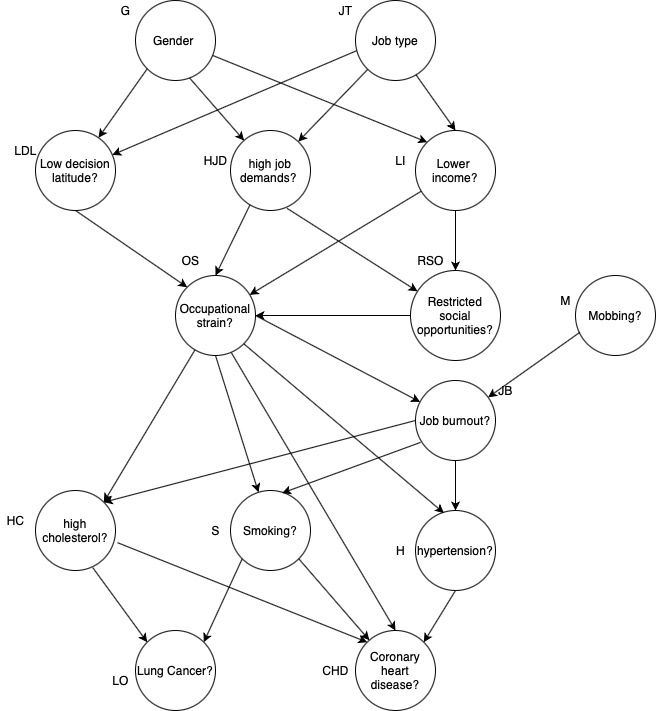
\includegraphics[width=0.8\textwidth]{Assets/BN_diseases.jpg}
    %\caption{BN of the use case}
    %\label{fig:my_label}
%\end{figure}

\subsubsection{Variables:}
\paragraph{Gender (G):} Gender has be selected has a root node with values "Male" and "Female". The reason behind it is that there is a proven distinction between men and women in reported levels of job strain and its consequences, specifically women reported research shows how women typically perceive higher levels of job strain than men. ~\cite{ref_article7}
\paragraph{Job type (JT):} We considered adverse job conditions as our second root node as, like the gender, are know to have an influence on strain levels. We defined active jobs as occupations with high demands combined and high control and passive jobs as low demands and low controls occupations. Both active and passive jobs are related to different maladaptive behaviors (i.g. smoking intensity has been reported as higher in passive jobs). ~\cite{ref_article3}
\paragraph{Mobbing (M):} A third root node was chosen, mobbing (workplace psychological and behavioral aggression) as a possible cause for job burnout.  
\paragraph{Low decision latitude (LDL) and High Job Demands (HJD):} According to the "Demands-Control Model" the combination of low decision-making power and high job requests produce conditions for high job strain. ~\cite{ref_article6}
\paragraph{Lower Income (LI):} According to the "Effort-Reward Imbalance", refers not so much to an income received but an income perceived as lower than due compared to the effort put into the job. ~\cite{ref_article6}
\paragraph{Restricted social Opportunities (RSO):} We considered restricted social opportunities as a secondary variable caused by the low income and which could influence job stress. Social isolation was later added to demand-control scheme ~\cite{ref_article5} as contributing factor to high strain and then proven to increase Cardiovascular Diseases (CVD) prevalence risk ~\cite{ref_article2} 
\paragraph{Occupational Strain (OS):} Job strain can be defined as a state of physical and mental strain caused by an imbalance between strict job requirements and an inadequate ability to adapt and cope ~\cite{ref_article1}. 
\paragraph{Job Burnout (JB):} Job burnout is a state of stress characterized by emotional exhaustion, cynicism, negative self-evaluation and mental disorders. OS is seen as a predecessor of JB. ~\cite{ref_article1}
\paragraph{High Cholesterol (HC), Smoking (S) and Hypertension (H):} We selected these three variables among a frame of possible CHD risk factors which could mediate between occupational strain occurrence. ~\cite{ref_article6}
\paragraph{Coronary heart disease (CHD):} CHD refers to a more specific condition among Cardiovascular Diseases which possible physiological factors risk factors have been linked to psychological imbalances due to a non-favorable work environment.  
\paragraph{Lung Cancer (LC):} This last variable has been added as a possible consequence due to High Cholesterol and Smoking incidence. Cigarette smoking and dietary factors are, in fact, known as dominant risk factors for lung cancer. ~\cite{ref_article8} 

\subsection{Queries}
\subsubsection{Prior marginal:}
As prior marginals we decided to test the probability of being a woman and having a coronary heart disease: Pr(G $\wedge$ CHD).
\\
%table%
\begin{table}
\centering
\caption{Prior marginal}\label{tab1}
\begin{tabular}{p{1.2cm} p{1.2cm} p{1.2cm}}
% \hline
CHD &  G &  Pr\\
\hline
F & {F} & 0.309734\\
F &  {T} & 0.148416\\
T & {F} & 0.352499\\
T & {T} & 0.157501\\
% \hline
\end{tabular}
\end{table}\\
Prior marginal query suggests that females are more likely to be diagnosed with CHD than males in general. On the other hand they are also more likely to be negatively diagnosed than males.
\subsubsection{Posterior marginal:} 
Evidence shows that heavy smokers are more likely to report high job demands ~\cite{ref_article3} . Assuming, as stated above, that smoking behaviors can be a mediating factor between job strain and coronary heart disease we want to test the probability of developing the disease given evidence of this two conditions happening together: Pr(CHD = T $\mid$ S = T, HJD = T).
\\
%table%
\begin{table}
\centering
\caption{Posterior marginal}\label{tab2}
\begin{tabular}{p{1.2cm} p{1.2cm}}
%\hline
CHD &  Pr\\
\hline
F &  0.665808\\
T &  0.334192\\
%\hline
\end{tabular}
\end{table}
\\
It is more likely not to develop a coronary heart disease (66.58\%) than to develop it (33.41\%) given a person is a heavy smoker and more likely to have high job demands. 

\subsubsection{MPE:}
A part from smoking, the other two mediating factors are high cholesterol and hypertension. We want to verify the most likely events to occur knowing that at least one of them or both are true.
\\
%table%
\begin{table}
\centering
\caption{MPE}\label{tab3}
\begin{tabular}{p{0.6cm} p{0.6cm} p{0.6cm}p{0.6cm}p{0.6cm}p{0.6cm}p{0.6cm}p{0.6cm}p{0.6cm}p{0.6cm}p{0.6cm}p{0.6cm}p{0.6cm}p{0.6cm}p{0.6cm}}
%\hline
G & JT & HJD & LI & RSO & M & JB & H & LDL & OS & LC & HC & S & CHD & p
\\
\hline
F & F & T & F & T & F & F & T & F & T & T & T &
   F & F & 0.002031\\
T & F & T & T & F & T & T & F & T & F & F & T & T &
   T & 0.001971\\
T & T & T & T & T & T & T & T & T & F & T & T & T & T & 0.002603\\
%\hline
\end{tabular}
\end{table}
\\
The most likely instantiation of MPE given that a person has a HC or H is when a person has both with a probability of 0.2603\%. Such a person is a male, has an active job high job demands, low income, restricted social opportunities, has experienced mobbing, experienced job burnout, low decision latitude, low occupational strain, has lung cancer, smokes and has a heart coronary disease. 

\subsubsection{MAP:} 
Restricted social opportunities, and so perceived social support, are influenced by the income, which we assume to be different considering the gender and the job type, and can influence the probability of job strain to occur. Given evidence of OS being T and RSO being F we want to verify the most likely instantiations for the G and the JT. \\

%table%
\begin{table}
\centering
\caption{MAP}\label{tab3}
\begin{tabular}{p{1.2cm} p{1.2cm} p{1.2cm}}
%\hline
G & JT & Pr\\
\hline
T & {T} & 0.050574\\
%\hline
\end{tabular}
\end{table}


The MAP query suggest the is most likely to be a man and have and active job type when there are occupational strain and restricted social opportunities present (p = 0.051).

\subsubsection{d-Separation:}
Given evidence of both Occupational strain and mobbing being T, we want to test weather both diseases are independent from the gender and job type.  Therefore, we tested if set of variables {G, J} are d-separated from {CHD, LC} by {OS = T, M = T}. The d-separation proved to be T. 













